\documentclass[12pt]{article}
\usepackage[utf8]{inputenc}
\usepackage{parskip}
\usepackage[spanish]{babel}
\usepackage{amsmath, amssymb}
\usepackage{graphicx}
\usepackage{makecell}
\usepackage{geometry}
\usepackage{caption}
\usepackage{float}
\usepackage[hidelinks]{hyperref}


% --------------------- Comandos para pie de página ---------------------
\usepackage[backend=biber, style=apa]{biblatex}
\addbibresource{referencias.bib}
\usepackage{hyperref}
\usepackage{url}
\usepackage{csquotes}

\makeatletter
\g@addto@macro{\UrlBreaks}{\UrlOrds}
\makeatother

\renewcommand{\footnoterule}{%
  \kern -3pt                         % Espacio vertical sobre la línea
  \hrule width \textwidth height 0.4pt % Ancho total de la página y grosor
  \kern 2.6pt                        % Espacio vertical debajo de la línea
}
% -----------------------------------------------------------------------

\addbibresource{referencias.bib}
\geometry{letterpaper, margin=2.5cm}
\setlength{\parskip}{1em}

\begin{document}
\begin{titlepage}
\begin{center}
    % Logos
    \begin{minipage}{0.3\textwidth}
        
\includegraphics[width=0.8\linewidth]{imagenes/UNAM_Logo.png}
    \end{minipage}\hfill
    \begin{minipage}{0.4\textwidth}
        \begin{center}
            \textbf{\Large Universidad Nacional Autónoma de México}\\[0.2cm]
            \textbf{Facultad de Ciencias}\\[0.2cm]
        \textbf{Bases de Datos}
        \end{center}
    \end{minipage}\hfill
    \begin{minipage}{0.3\textwidth}
        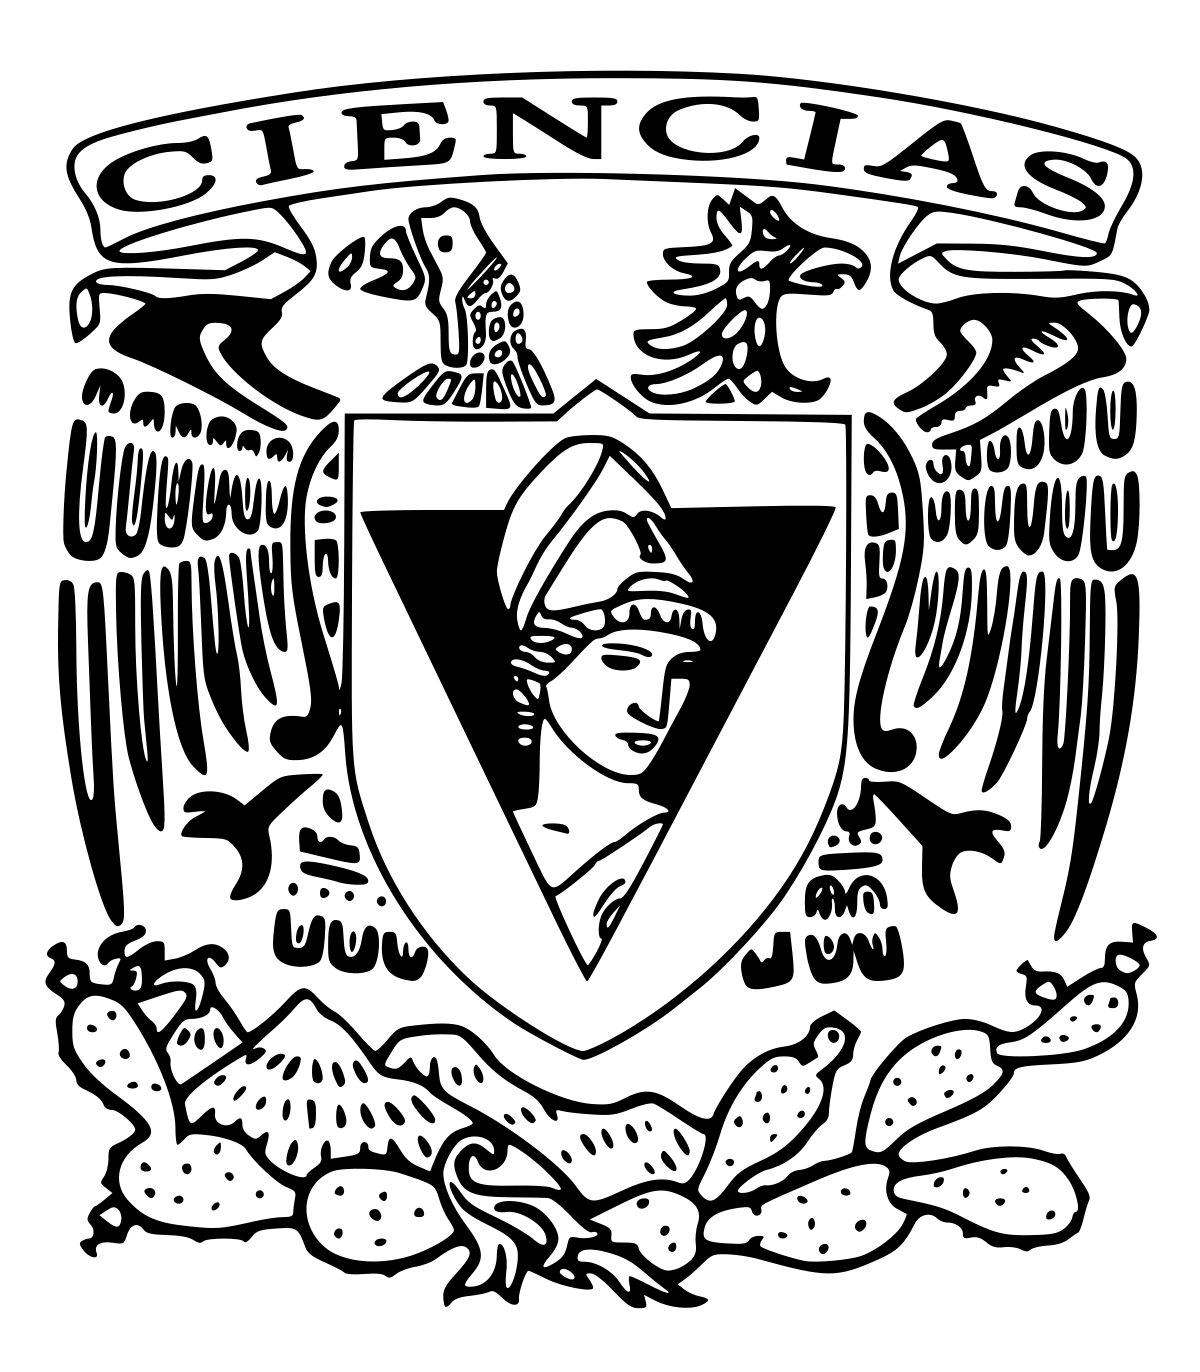
\includegraphics[width=0.8\linewidth]{imagenes/Logo_FC.png}
    \end{minipage}
    \vspace{3cm}
    \textbf{\large Tarea 1}\\
    Licenciatura en Ciencias de la Computación\\
    Profesor: Gerardo Avilés Rosas \\
    \vspace{2cm}
    \textbf{Integrantes: }\\
    Cisneros Tenorio Diego Alexander\\
    Nuñez Ruiz José Manuel \\
    Olmos Ortiz Andrea Lucia\\
    Reynoso Ascencio Alexa \\
    Vega Navas Saúl \\
    \vspace{2cm}
    \textbf{Fecha de entrega: } 08 de septiembre del 2026
    \vfill
\end{center}
\end{titlepage}
\tableofcontents
\newpage

% Preguntas

 \section{Conceptos generales de bases de datos}

\subsection*{a.}

\addcontentsline{toc}{subsection}{Inciso a}

\textbf{Explica las características fundamentales del enfoque de bases de datos frente al uso de hojas de cálculo. ¿Qué limitaciones enfrentan las hojas de cálculo cuando se trata de escalabilidad, integridad y consistencia de datos? Describe al menos dos escenarios concretos:}
\begin{itemize}
    \item \textbf{Uno donde no sea adecuado usar hojas de cálculo.}
    \item \textbf{Otro donde sí sea preferible optar por ellas. Justifica cada caso.}
\end{itemize}

A diferencia de los sistemas de bases de datos, las hojas de cálculo están principalmente diseñadas para el análisis numérico y la presentación de información en un formato de tabla bidimensional; además, ofrecen accesibilidad por completo a quien accede a éste, un usuario a la vez, por lo que carecen de sistemas de restricción de acceso, sino que los archivos son cargados por completo y abiertos a lectura-escritura. Puesto que no tienen un enfoque en el almacenamiento estructurado y relacional, presentan limitaciones en cuanto a:
\begin{itemize}
    \item \textbf{Escalabilidad:} Conforme aumenta la cantidad de datos almacenados, el rendimiento de la se puede ver considerablemente afectado puesto que no está diseñado para almacenar grandes volúmenes de datos. Además, aplicaciones como Excel tienen un límite definido en la extensión manejable de las dimensiones. Por otra parte, no se pueden añadir relaciones con otras tablas aplicando integridad referencial, puesto que las tablas no cuentan con llaves primarias y foráneas que puedan vincularlas entre sí.
    \item \textbf{Integridad:} El acceso para lectura y escritura de datos no cuenta con tecnología de autenticación, sino que tiene un enfoque de total accesibilidad de escritura; esto permite modificar cualquier parte del archivo, dejándolo expuesto a errores si éstos se ingresan manualmente. Además, si el sistema sufre de un apagón mientras el archivo es manipulado, o si se trata de sobreescribir por dos fuentes concurrentes, se corre el riesgo de que éste se corrompa por completo.
    \item \textbf{Consistencia de datos:} No se puede validar un tipo de dato en particular para una columna, sino que se puede ingresar texto libre en cualquier celda, dando pie fácilmente a violaciones a la propiedad de integridad puesto que los datos pueden ser almacenados en cualquier formato.
\end{itemize}

\textbf{Escenarios puntuales:}
\begin{itemize}
    \item \textbf{No utilizar hojas de cálculo:} Si en un hospital se busca desarrollar un sisteam de gestión de los datos de los pacientes no es viable desarrollar éste con una hoja de cálculo, puesto que toda la información de la insitución no solo puede quedar expuesta a perderse ante incidentes como apagones si se está manipulando, sino que también es visible para cualquier empleado con cualquier acceso al sistema, puesto que el archivo es de libre escritura y no integra roles de usuario $-$si bien esto se puede agregar en cierta medida con restricciones a nivel de OS y una aplicación de gestión, el archivo sigue vulnerable ante el superusuario$-$.
    \item \textbf{Mejor utilizar hojas de cálculo:} En un caso donde se quiera organizar una cantidad de reducida de datos que no se consideren como críticos (p.ej. contraseñas) y con un único tipo de acceso y que sea total, como en un registro personal de itinerario o de finanzas, es preferible hacer uso de una herramienta de hojas de cálculo dada su interfaz amigable a comparación del proceso de levantamiento de un sistema de base de datos.
\end{itemize}

 \subsection*{b.}
\addcontentsline{toc}{subsection}{Inciso b}

\textbf{b. Supón que una empresa en crecimiento necesita implementar un sistema de administración de bases de datos (SMBD) para centralizar su información operativa (ventas, clientes, inventario y logística). Elige dos posibles soluciones (p.e., PostgreSQL, Oracle, MySQL, SQL Server, etc.) y compara sus ventajas y desventajas en términos de: rendimiento ante grandes volúmenes de datos; escalabilidad a futuro; costos de licenciamiento y mantenimiento; soporte técnico y comunidad. Con base en tu análisis, argumenta cuál solución recomendarías y por qué.}

Para realzar este análisis, se realizará una comparativa entre los sistemas manejadores de bases de datos (SMBD): PostgreSQL y Oracle. Particularmente, como Oracle tiene una versión gratuita y una versión de pago, que no es fija y depende de las necesidades del sistema, para algunos criterios se tomaran en cuenta ambos y se compararán con PostgreSQL. El análisis se realizará en base a los siguientes 4 criterios.

\begin{itemize}
\item \textbf{Rendimiento del sistema ante grandes volúmenes de datos:} Tanto Oracle en su versión de pago y PostgreSQL están diseñadas para operar con grandes volúmenes de datos. Cabe mencionar que la versión gratuita de Oracle está limitada en cuanto a los recursos disponibles, teniendo un límite de almacenamiento de 12 GB.
\item \textbf{Escalabilidad: } Del mismo modo, Oracle en su versión de pago y PostgreSQL, son buenas opciones, ya que, por un lado, las licencias de pago de Oracle, permiten que el sistema sea tan amplio como la necesidad lo requiera, mientras que a nivel de Software, PostgreSQL, no ofrece ninguna limitante en cuanto a memoria RAM o número de procesadores que pueden ser destinados al mantenimiento del sistema, por lo que ambos sistemas son escalables. Cabe mencionar que la versión gratuita de Oracle impone limitaciones considerables a nivel de recursos, permitiendo usar un máximo de 2 procesadores y 2 GB de RAM.
\item \textbf{Costos de licenciamiento y mantenimiento: } Ambos requieren un costo de infraestructura para el almacenamiento de los datos; sin embargo, en Oracle se necesita pagar una licencia para sostener su funcionamiento con el aumento de los datos y una licencia de mantenimiento para mantener el software actualizado, mientras que PostgreSQL es un software completamente gratuito.\
\item \textbf{Soporte técnico y comunidad.} Con la licencia de pago de Oracle, se ofrece un soporte técnico especializado en resolver cualquier problema con el manejo del software, mientras que PostgreSQL, al ser de código abierto, no ofrece un soporte técnico directo, pero cuenta con una amplia comunidad para solucionar cualquier problema que pueda surgir; el soporte y mantenimiento del sistema queda en manos de la empresa.
\end{itemize}
Del análisis anterior, consideramos que Oracle, con su licencia de pago, presenta ventajas considerables al momento de realizar un mantenimiento al sistema y para solucionar problemas técnicos; sin embargo, por el costo elevado de sus licencias, consideramos que la mejor opción para una empresa en crecimiento es PostgreSQL, ya que no requiere un costo extra por manejo de software, ofrece una gran escalabilidad y tiene una gran capacidad para sostener los datos originados por la empresa con su crecimiento.


 \subsection*{c.}
\addcontentsline{toc}{subsection}{Inciso c}
\textbf{Una empresa de logística necesita adaptar su sistema de base de datos para incluir nuevas
funcionalidades, como el seguimiento en tiempo real de paquetes y una nueva categoría de
clientes corporativos. Antes de realizar estos cambios, el equipo de desarrollo debe considerar los
niveles de independencia de los datos. Responde lo siguiente:}

\begin{itemize}
    \item \textbf{¿Qué riesgos podrían surgir sí no existe independencia lógica entre el diseño conceptual y las aplicaciones que consumen los datos?}

    Si no existe independencia lógica, al modificar los esquemas conceptuales de la base de datos se obliga a modificar los esquemas externos y el código de las aplicaciones que consumen la información. En la empresa de logística, al añadir la nueva categoría de clientes corporativos (mediante tablas o atributos del esquema conceptual), se requerirá forzosamente reescribir y recompilar los programas de aplicación. Esto genera un incremento en los tiempos y costos de mantenimiento, además pueden ocurrir fallos en la producción si la aplicación no se actualiza a tiempo.
    
    \item \textbf{¿Qué problemas operativos aparecerían sí no se logra la independencia física, especialmente en términos de almacenamiento y rendimiento?}
    
    Si no se logra la independencia física, al momento de querer modificar el esquema interno, tendremos necesariamente que modificar el esquema conceptual y se romperán las consultas de los programas de aplicación.

    Enfocándonos en la empresa de logística, si no se logra la independencia física al querer aplicar nuevas funciones como el seguimiento en tiempo real de paquetes, se presentarán varios problemas operativos. En cuestión de almacenamiento, no se podrá cambiar la ubicación de los datos en disco, ni comprimir, dividir o fusionar registros para optimizar el espacio sin alterar las aplicaciones. Y hablando del rendimiento, no se podrán crear estructuras o rutas de acceso adicionales para acelerar las búsquedas de paquetes, generando respuestas lentas e ineficientes.
    
    \item \textbf{Proporciona un ejemplo realista en el que un cambio físico no afecte la lógica del sistema, y otro donde un cambio lógico pueda impactar múltiples aplicaciones sí no se gestiona adecuadamente.}

    \begin{itemize}
        \item Crear una ruta de acceso sobre el código del paquete para buscar de manera rápida el rastreo en tiempo real sin tener que cambiar la consulta de la aplicación.
        \item Agregar la entidad de clientes corporativos modificando tablas existentes; si no se abstrae mediante un esquema externo, este cambio romperá los programas de aplicación que no utilicen ese dato.
    \end{itemize}
\end{itemize}
 


 \addcontentsline{toc}{subsection}{Inciso d}

\subsection*{d.}

\textbf{Describe el papel que tienen los Sistemas Manejadores de Bases de Datos (SMBD) en el enfoque de bases de datos.}\\
Un Sistema Manejador de Bases de Datos es el software que proporciona cuatro herramientas esenciales para el manejo de datos:
\begin{itemize}
    \item \textbf{Definir:} Permite definir la lógica y estructura de los datos, esto es, sus tipos, restricciones y relaciones entre ellos.
    
    \item \textbf{Construir:} Es el proceso de almacenamiento de los datos físicamente, manejado por el SMBD.
    
    \item \textbf{Manipular:} Como su nombre lo dice, manipula los datos mediante inserciones y actualizaciones de datos. Además incluye la función de consulta de estos.

    \item \textbf{Compartir:} Permite que diversos usuarios puedan interactuar con la Base de Datos paralelamente, es decir, de forma simultánea. 
    
\end{itemize}

\textbf{¿Por qué consideramos que es importante (o no) que un administrador de bases de datos conozca las características de un SMBD?}

Consideramos que, en efecto, el Administrador de Bases de Datos (DBA) debe conocer las características de un SMBD.
El administrador de bases de datos se encarga principalmente de las siguientes tareas:
\begin{enumerate}
    \item \textbf{Mapear el modelo lógico al físico:} Esto es, se encarga de plasmar los tipos, restricciones y relaciones entre los datos físicamente en la memoria.
    \item \textbf{Implementar copias de seguridad:} Para salvaguardar la integridad de los datos utiliza copias de seguridad que permitan restablecer los datos en casos de contingencias por algún incidente.
    \item \textbf{Optimización de rendimiento:} Al hacer la traducción del modelo lógico al físico suele optimizar la distribución de memoria a las tareas más utilizadas por los usuarios.
    \item \textbf{Mantenimiento y actualizaciones:} Suele actualizar el software y aplicar parches de seguridad al sistema.
\end{enumerate}

Primero debemos notar que es esencial que el administrador de bases de datos conozca su SMBD específico, pues cada software puede diferir en su implementación. Sin embargo, mi argumento se sostiene principalmente por la tarea del mapeo del modelo lógico al físico, pues es en este aspecto donde es imperativo que el DBA domine el tema.
Ya que será el encargado de crear las relaciones en el medio de almacenamiento, las restricciones y optimizar el uso de la base de datos, lo que requiere considerar qué relaciones serán más usadas en las consultas de los usuarios.\\
Si el DBA no comprende las características del SMBD no podrá establecer la correspondencia conceptual/física eficiente o, más aún, podrá violar la independencia física de los datos, es decir, que cambios en el nivel físico afecten el nivel lógico. Además, si no domina el esquema, podrá no definir correctamente las relaciones entre las entidades, la elección de los tipos de datos para cada atributo planteado y las restricciones de integridad, por lo que no representaría fielmente el ``Mini mundo'' planteado por el diseñador, permitiendo inconsistencias en los datos almacenados. Finalmente estas limitaciones serían un impedimento para la escalabilidad del sistema en un futuro.


 \addcontentsline{toc}{subsection}{Inciso e}

\subsection*{e.}

\textbf{Durante el desarrollo de un nuevo sistema empresarial surge una discusión entre quienes consideran que la base de datos debe diseñarse pensando únicamente en las necesidades actuales y quienes proponen anticipar futuros requerimientos. Analiza esta situación relacionándola con el ciclo de vida de una base de datos y argumenta cómo las decisiones tomadas durante las etapas iniciales pueden influir en el mantenimiento, evolución y costo del sistema a largo plazo.}\\ \\
El argumento para diseñar el sistema pensando únicamente en los requerimientos actuales sería ahorrar tiempo en la fase de diseño, para poder implementar la base de datos lo más pronto posible.\\ \\
Sin embargo, las decisiones tomadas durante la fase de diseño determinarán qué tan costoso será modificar el sistema después. Anticiparse a las necesidades predecibles futuras permite que durante el mantenimiento y las futuras intenciones de escalar la base de datos, los cambios realizados no afecten los datos históricos ni los sistemas que ya funcionan sobre el diseño original, evitando costos elevados en migraciones de datos y reescritura de aplicaciones, además de posibles interrupciones en el funcionamiento del sistema.
 \subsection*{f.}
\addcontentsline{toc}{subsection}{Inciso f}

\begin{itemize}
    \item \textbf{Investiga qué es la redundancia de datos.}
    
    La redundancia de datos es duplicar o almacenar información múltiples veces, dentro de una base de datos o sistemas de archivos.
    \item \textbf{¿Cuál sería la diferencia entre redundancia de datos controlada y no controlada? Proporciona un ejemplo claro de cada tipo.}
    \begin{enumerate}
        \item \textbf{Redundancia no controlada:} La información se duplica de forma desorganizada e independiente entre distintos archivos, sin que el sistema valide o controle los cambios.
        
        \textbf{Ejemplo:} En un sistema universitario, la oficina de inscripciones y la de contabilidad guardan archivos independientes del mismo estudiante. Si el alumno cambia de domicilio, la dirección puede actualizarse en un archivo pero omitirse en el otro, o registrarse con errores tipográficos distintos en cada lugar (como fechas de nacimiento diferentes).
        
        \item \textbf{Redundancia controlada:} Se duplican los datos de manera intencionada y planificada dentro del diseño del sistema, donde el SMBD realiza verificaciones automáticas para garantizar que los datos siempre coincidan.
        
        \textbf{Ejemplo:} Guardar a propósito el nombre de un alumno junto con su calificación en el historial de materias aprobadas. Para que el sistema pueda mostrar el reporte de calificaciones rápidamente sin tener que ir a buscar el nombre a la tabla de alumnos cada vez. Para evitar inconsistencias, el SMBD se encarga automáticamente de validar que el nombre asignado al reporte coincida siempre con el alumno registrado en la base de datos principal.
    \end{enumerate}
    \item \textbf{¿Por qué la redundancia no controlada suele ser un problema para la integridad y consistencia de los datos?}
    
    La redundancia no controlada es problemática porque, al duplicar la información de forma independiente en múltiples archivos, genera inconsistencias cuando los datos cambian y solo se actualizan en un lugar pero se omiten en los demás, dejando al sistema en un estado donde las fuentes no coinciden. Además, al requerir la captura manual e independiente de un mismo dato en varios sitios, incrementa significativamente la probabilidad de cometer errores humanos o tipográficos. Todo esto  también implica una duplicación ineficiente de esfuerzo y un desperdicio de espacio de almacenamiento.
    
\end{itemize}
 \addcontentsline{toc}{subsection}{Inciso g}

\subsection*{g.}

\textbf{Imagina que formas parte del equipo de tecnología de una empresa aseguradora que gestiona información sobre pólizas, clientes, siniestros, evaluaciones de riesgo y cumplimiento normativo. Responde lo siguiente:}\\
\textbf{¿Cuáles son las principales responsabilidades del DBA en este contexto, considerando la necesidad de confidencialidad, trazabilidad y disponibilidad continua de la información?}

Las responsabilidades del DBA se centran principalmente en los clientes, siniestros y cumplimiento normativo de la empresa aseguradora, ya que como se mencionó en una pregunta pasada, el DBA se encarga de la administración en el nivel físico del sistema de bases de datos, que compone el mapeo, optimización, mantenimiento y seguridad de los datos. Así podremos dividir sus responsabilidades en las tres necesidades planteadas en la pregunta:

\begin{enumerate}
    \item \textbf{Confidencialidad:} Se encargará de proteger los datos, definiendo roles, permisos y privilegios de los usuarios de la empresa. Así se controlará quién sí y quién no puede acceder a la información de los clientes, siguiendo las normativas. Por ejemplo, si un cliente siempre debería tener el poder de revisar su información personal registrada, por otro lado un trabajador no debería poder conocer toda la información personal de los clientes, sin embargo, sí deberá conocer el historial de pólizas del cliente o información puntual que necesite.
    
    \item \textbf{Trazabilidad:} Se encargará de implementar una forma de conocer quién modificó qué dato, cómo y cuándo, de esta forma no habrá vacíos en la manipulación de las bases de datos. Esto se logrará a través de la correcta configuración de bitácoras de transacciones y auditorías del sistema.
    
    \item \textbf{Disponibilidad continua:} Permitirá que los usuarios de la base de datos, en este caso los empleados, consulten los datos del cliente de forma simultánea y que el SMBD soporte esta acción. Además requiere la planificación de respaldos, actualización y monitoreo de la base de datos por parte del DBA para que el sistema siga operando en caso de siniestros imprevistos, así como para implementar versiones de respaldo consistentes para recuperar la información ante cualquier adversidad que se presente.
\end{enumerate}

\textbf{¿Qué habilidades técnicas y conocimientos específicos (por ejemplo, manejo de datos sensibles, normativas como protección de datos personales, respaldo y recuperación ante desastres) son más críticos para este entorno?}

Creemos que las habilidades técnicas y conocimientos mencionados en la pregunta efectivamente pertenecen a las habilidades y conocimientos más críticos en el entorno, sin embargo, considero que la trazabilidad de los datos y la disponibilidad continua también pertenecen a este conjunto de conocimientos importantes. Desarrollaré cada punto en particular y explicaré por qué creo que son esenciales y ninguna puede faltar:

\begin{enumerate}
    \item \textbf{Manejo de datos sensibles y normativas como protección de datos personales:} Primeramente, por cuestiones legales los clientes tienen como derecho la protección de sus datos, por ejemplo, en México existe la ``Ley Federal de Protección de Datos Personales en Posesión de los Particulares'' que estipula que cualquier empresa debe proteger tus datos personales. Así que es imperativo que la empresa desarrolle (en particular el o los DBA) la confidencialidad como se explicó en la pregunta pasada.
    
    \item \textbf{Respaldo y recuperación ante desastres:} Ante cualquier adversidad contra el sistema de base de datos, el sistema debe ser capaz de tener una copia de seguridad del momento anterior a este para garantizar la integridad de los datos y si se interrumpió alguna transacción esta vuelve a su estado original para realizarla exitosamente. Sin esto la empresa sufriría con cualquier incidente (por ejemplo, la descompostura de algún servidor) y podría tener una complicación grave que la pueda llevar a la quiebra.
    
    \item \textbf{Trazabilidad y disponibilidad de datos:} La trazabilidad permite saber quién modificó qué, cuándo y dónde, esto es vital para detectar fraudes o accesos no autorizados de los empleados, sin esto el sistema podría ser vulnerado desde adentro. Por otra parte la disponibilidad es esencial para que los múltiples empleados puedan consultar, por ejemplo, pólizas al mismo tiempo sin que el sistema genere fallas o vulnere la integridad de los datos.
\end{enumerate}

\textbf{Si el DBA no ejecuta consultas directamente, ¿por qué sigue siendo necesario que comprenda el modelo lógico de la base de datos? Justifica tu respuesta considerando la importancia de la integridad de los datos en procesos como la evaluación de riesgos o la detección de fraudes.}

Como se planteó anteriormente en el inciso d) el DBA necesita entender totalmente el modelo lógico para realizar una implementación correcta y óptima de este, en este caso nos concentraremos en justificar esto con respecto a la integridad de los datos en el contexto de la empresa aseguradora, es decir, con la evaluación de riesgos o la detección de fraudes.

Supongamos que el DBA no comprende correctamente el modelo lógico de la base de datos así que cuando implementa las restricciones otorga poder excesivo a algunos empleados, por ejemplo, poder modificar los datos de los clientes y el historial de pagos. Así, un empleado toma una póliza vencida, la pone a nombre de un cliente y cambia la fecha para que esté activa; después crea un siniestro falso, uno por \$25,000 pesos de algún accidente, la transferencia se hace y al tener el poder de modificación del historial de pagos elimina el pago final, de esta manera la empresa cuando se dé cuenta del desfalco no podrá encontrar quién lo hizo ni exactamente cómo pasó. Este es un ejemplo de cómo un DBA que no domine el modelo lógico podría pasar por alto restricciones esenciales para una empresa. En el caso de la evaluación de riesgos el empleado fraudulento podría modificar alguna condición de un cliente para que la póliza se cobre a un precio más bajo, estos ejemplos atentan contra la integridad de los datos, creando contradicciones al imponer datos falsos.

Por estos motivos, aunque el DBA no ejecute consultas o diseñe el modelo lógico, necesita comprenderlo para no cometer errores y realizar su trabajo correctamente.

 \addcontentsline{toc}{subsection}{Inciso h}

\subsection*{h.}

\textbf{A lo largo del tiempo han existido diversos modelos de datos, como el modelo jerárquico, el modelo de red, el modelo relacional, el modelo orientado a objetos y los modelos NoSQL (llave-valor, documento, columnares, grafos).Responde lo siguiente:}

 \noindent \textbf{Elabora una tabla comparativa entre al menos cuatro modelos de datos, destacando sus principales características, ventajas, desventajas y casos de uso típicos.}
\begin{figure}[H]
    \makebox[\textwidth][c]{%
        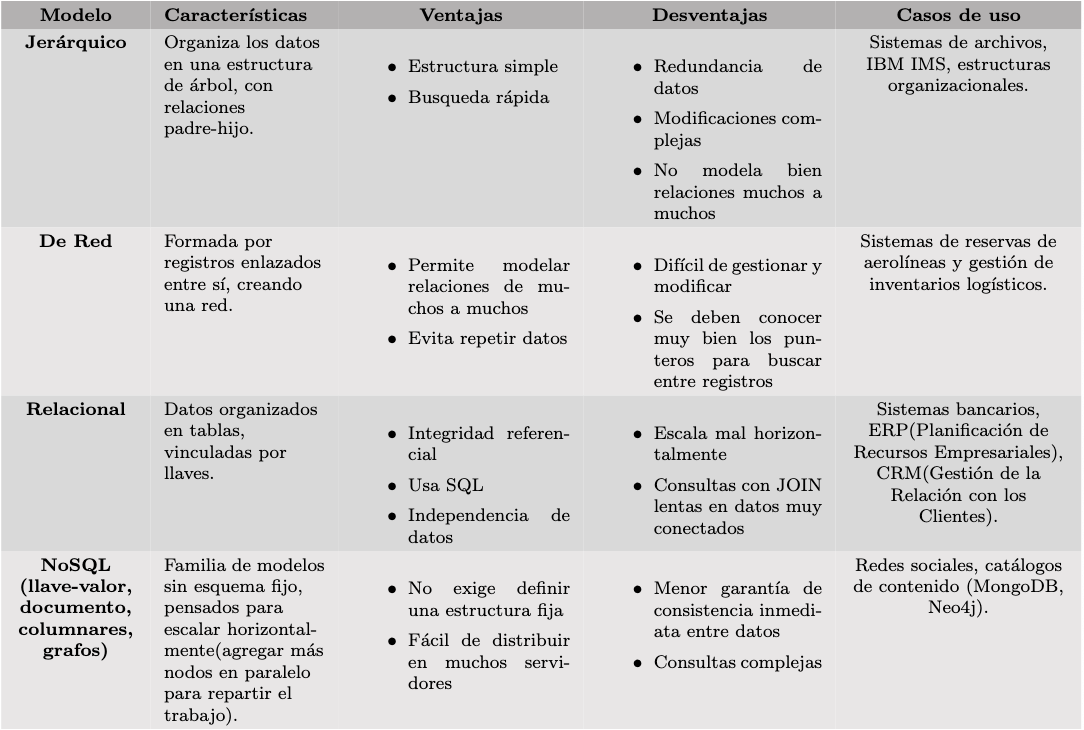
\includegraphics[width=1.2\linewidth]{imagenes/TABLA.png}%
    }
\end{figure}
\noindent \textbf{¿Por qué crees que el modelo relacional se convirtió en el más ampliamente adoption durante décadas?}

Al estar basado en la teoría de conjuntos y álgebra relacional, proporcionó una fomra estructurada de representar las relaciones entre los datos.

Ádemas, la creación de SQL como lenguaje estándar facilitó la formación de profesionales, estableciendo una forma común de trabajar con las bases de datos.

Por último, al permitir forzar la integridad y consistencia de los datos de forma declarativa, generó una gran confianza para su uso en aplicaciones empresariales, como sistemas bancarios y de comercio, que contribuyó a consolidarlo como el modelo dominante por décadas.

\textbf{¿En qué contextos actuales los modelos NoSQL superan al modelo relacional en eficiencia o flexibilidad? Justifica con ejemplos.}

Las bases de datos NoSQL ofrecen mayor rendimiento y adaptabilidad cuando se trabaja con grandes volúmenes de datos no estructurados.

Los principales contextos donde los modelos NoSQL destacan son:
\begin{itemize}
    \item Cuando existen grandes volúmenes de datos distribuidos con escrituras de alta frecuencia.
    \item Al manejar datos semiestructurados o no estructurados, como catálogos con atributos variables, bitácoras y eventos.
    \item En aplicaciones que requieren rapidez de respuesta en lecturas simples, como sesiones de usuario, caché o contadores.
    \item En entornos IoT, donde se presentan ingestas masivas de datos provenientes de múltiples dispositivos.
    \item En redes sociales, catálogos de productos y sistemas de recomendación con esquemas cambiantes.
    \item Durante procesos de analítica distribuida donde los datos se procesan en múltiples nodos.
    \item En proyectos donde el esquema evoluciona con frecuencia.
\end{itemize}

 \subsection*{i.}
\addcontentsline{toc}{subsection}{Inciso i}
\textbf{Una institución financiera necesita almacenar millones de registros relacionados con clientes, cuentas y transacciones. Aunque la capacidad de almacenamiento ya no representa una limitación importante, la organización sigue invirtiendo recursos en el diseño adecuado de sus bases de datos. Explica por qué la simple acumulación de datos no garantiza información útil y analiza la importancia de aspectos como organización, estructura, integridad y seguridad para el éxito de los sistemas de información.}

Diseñar una base de datos útil para un propósito especifico, requiere que los datos almacenados sean útiles para resolver dicho propósito. De este modo, los datos almacenados en una base de datos deben, en primer lugar, estar asociados con la cuestión a resolver y en segundo lugar, particularmente en bases de datos a gran escala y en crecimiento como en el caso de una institución financiera, se debe tener la capacidad de manipular dichos datos con facilidad, para extraer la información necesaria y cumplir con su propósito.

Para obtener información importante de una base de datos, se debe tener la capacidad de establecer relaciones entre los datos. Una colección de datos sin relaciones entre si, es una colección dispersa y difícil de interpretar, particularmente para este caso, si se tiene una colección con los datos de clientes, cuentas y transacciones, pero no se tiene la capacidad de relacionarlos entre si, se pierde la capacidad de obtener mayor información del conjunto de datos almacenados, como las cuentas y las transacciones que puede realizar un cliente.

Realizar un diseño adecuado para el almacenamiento de los datos, permite extraer información fiable, además de otorgar seguridad sobre la informacion obtenida. Para el diseño se debe considerar:
\begin{itemize}
    \item \textbf{Organización eficiente: } Es necesario tener una forma de almacenamiento en la que se puedan manipular y revisar los datos de manera eficiente. Particularmente en una base de datos enorme y creciente como la de una institución financiera, con múltiples consultas y modificaciones, es indispensable tener la capacidad de operar con la base de datos de forma rápida y evitar retrasos con la información proporcionada a los clientes.
    \item \textbf{Estructura adecuada: } Como se mencionó anteriormente, una colección de datos por si mismos no tienen la capacidad de proporcionar información adecuada. Por ello, es necesario darles una estructura correcta, con la que sea fácil consultarlos, y relacionarlos correctamente entre si para extraer la información necesaria y cumplan con su propósito.
    \item \textbf{Integridad: } Esta cualidad, permite establecer reglas para que los datos almacenados sean coherentes y garantizar que la información obtenida a partir de las relaciones entre datos sea consistente. Para el caso de una institución financiera, es de suma importancia que los datos almacenados tengan sentido, pues la existencia de datos corruptos sobre cuentas y transacciones realizadas por los clientes, puede ocasionar pérdidas económicas en el futuro. Por ejemplo, al realizar una transacción, es indispensable que el cliente tenga en su cuenta el monto suficiente para realizarla, sin esta restricción, el cliente puede realizar transacciones sin restricciones y ocasionarle pérdidas a la institución.
    \item \textbf{Seguridad: } Es indispensable tener un control sobre las operaciones que se pueden realizar sobre la base de datos y evitar vulnerabilidades que conlleven una perdida de información. En particular, para una institución financiera, se vuelve indispensable, pues perder o filtrar información sobre sus clientes implicaría una perdida económica y de fiabilidad para la institución.
\end{itemize}
Una colección de datos almacenada sin un diseño adecuado es una base de datos vulnerable y propensa a errores futuros. Por esta razón, invertir en el diseño de la base de datos, es una inversión para evitar pérdidas en el futuro y para obtener información consistente, lo cual es fundamental en cualquier institución.

 \addcontentsline{toc}{subsection}{Inciso j}

\subsection*{j.}

\textbf{Supón que deseas crear una aplicación para gestión hospitalaria. Considera cada una de las desventajas indicadas en el documento “Purpose of Database Systems”, cuando se administran los datos en un sistema de archivos. Discute la relevancia de cada uno de los puntos indicados, con respecto a la relevancia de cada desafío en el contexto de la gestión de datos de pacientes: historial médico, diagnósticos, tratamientos, citas, acceso a registros médicos, médicos, especialidades, entre otros.}

En la lectura ``Purpose of Database Systems'' \cite{PurposeDatabaseSystems} nos dan ejemplos en un contexto universitario mayormente, de por qué el sistema de archivos no es eficiente y puede traer muchos problemas a cualquier establecimiento que necesite organizar sus datos. En este caso, en el contexto de un hospital y la gestión hospitalaria, procederé a particularizar cada punto para mapear los siete desafíos tratados en la lectura, pero en este contexto específico, centrándome en explicar con ejemplos y notando que cada punto es vital para el hospital.

\begin{enumerate}
    \item \textbf{Redundancia e inconsistencia de datos (Data redundancy and inconsistency):} La redundancia de datos de un paciente es extremadamente peligrosa en el contexto de un hospital. Supongamos que un paciente llega a un hospital por primera vez a la especialidad de urgencias, su malestar es tratado, sus datos son recolectados y se le dirige ahora a cardiología; en esta especialidad se le vuelven a recolectar los datos y se le da un diagnóstico y tratamiento. Días después, el paciente llama para actualizar su número telefónico, pero al no haber centralización de los datos, esta actualización solo se le notifica a la especialidad de urgencias. Esto genera una \textbf{inconsistencia de datos}. Así que, si hay alguna complicación o por alguna razón una de las especialidades necesita del paciente, puede que no tenga el teléfono actualizado del paciente y se tenga que buscar en otras especialidades. Esto hace no solo ineficiente la comunicación, sino que pone en riesgo la salud y la vida de los pacientes.

    \item \textbf{Dificultad en el acceso de datos (Difficulty in accessing data):} Aunque pareciera a primera vista que este punto no afecta directamente la integridad de los pacientes, en realidad sí lo hace de forma indirecta, ya que la dificultad en obtener datos de un hospital ralentiza su funcionamiento y no permite que se atienda a la cantidad de pacientes necesarios, o peor aún, podría atentar contra la salud de los pacientes. Supongamos que el hospital requiere conocer a todos los pacientes a los que se les administró un fármaco, digamos el fármaco X, pero sus datos están almacenados en un sistema de archivos, por lo que no existe un programa que satisfaga esta tarea de manera inmediata. Debido a esto, o se debe buscar manualmente en cada archivo o se debe programar la consulta desde cero; ninguna opción es eficiente y ambas requerirán mucho tiempo. Esto puede ser muy peligroso si la razón por la que se necesita conocer a qué pacientes se les administró el fármaco X es porque este podría provocar reacciones alérgicas no identificadas antes. Esta es una de las diversas adversidades que pueden surgir por una mala elección del método de almacenamiento de datos.

    \item \textbf{Aislamiento de datos (Data isolation):} Aquí podemos ver un mapeo casi directo de lo dicho en la lectura ``Purpose of Database Systems'' \cite{PurposeDatabaseSystems} en la parte de aislamiento de datos. Si cada especialidad del hospital está programada por distintos equipos, al querer escribir un nuevo programa (como el del punto anterior para obtener la lista de los pacientes a los que se les administró el fármaco X), implementar dicho programa en las diversas especialidades sería un problema aún peor de lo que se pensaba.

    \item \textbf{Problemas de integridad (Integrity problems):} Este punto parece similar al anterior, pero en este caso nos centraremos en la constante actualización del sistema, en particular para implementar restricciones de consistencia. Por ejemplo, si el hospital adquiere un nuevo medicamento, este tendrá la restricción de dosis máxima segura, digamos 50 mg. Como este fármaco se utilizará en prácticamente todas las especialidades del hospital, se necesitará implementar esta restricción; sin embargo, nos enfrentamos al problema de que cada especialidad tiene su propia implementación independiente, por lo que su aplicación coordinada será sumamente complicada y se podría vulnerar la integridad de los datos.

    \item \textbf{Problemas de atomicidad (Atomicity problems):} Este es uno de los problemas más críticos que debe tener en cuenta el hospital, ya que debe tener un plan de acción ante fallas que, como en cualquier otro sistema computacional, pueden ocurrir. El concepto plantea que las transacciones o movimientos deben ser atómicos, es decir, que se realiza toda la transacción o no se hace nada de ella. Supongamos que se le va a asignar un quirófano y un médico a una cirugía de apéndice, pero en ese momento ocurre una falla eléctrica en el hospital, por lo que la asignación queda incompleta (el médico tiene asignado el quirófano pero el sistema no registró qué cirugía va a realizar). En este caso, el sistema debería tener una forma de volver al estado anterior a la asignación para no crear incongruencias; en otro caso, la cirugía tendría que ser aplazada o incluso se podría perder la información del turno, lo cual atenta contra la salud del paciente.

    \item \textbf{Anomalías de acceso concurrente (Concurrent-access anomalies):} Este punto estipula que en cualquier sistema la concurrencia de usuarios (el uso compartido del sistema por múltiples usuarios al mismo tiempo) es muy común y va cada vez más a la alza. Por ello, el sistema de un hospital debería tener la capacidad de que sus empleados puedan acceder a los datos de un paciente o trabajador al mismo tiempo sin que se generen incongruencias. Por ejemplo, si el departamento administrativo del hospital y una especialidad médica necesitan modificar la información de un paciente al mismo tiempo (digamos que la administración actualiza su número telefónico y el médico registra una nueva alergia detectada), sin un control de concurrencia podría pasar que ambos guarden su cambio sobre el mismo estado anterior, sobrescribiendo la información de la primera modificación guardada. En el peor de los casos, se perdería la alergia que el doctor acaba de diagnosticar sobre el paciente.

    \item \textbf{Problemas de seguridad (Security problems):} Este podría ser el punto más intuitivo u obvio, pero no por ello es menos importante. El sistema debe regular qué personal puede acceder a qué tipo de datos. Por ejemplo, el doctor puede acceder a los datos médicos generales del paciente, junto a sus tratamientos, citas y médicos asociados, sin embargo, no debería poder modificar sus datos personales administrativos como su número telefónico, correo o teléfonos de emergencia. Pero ya que la aplicación sigue un anticuado sistema de archivos muy específico para cada problema, cualquier restricción de seguridad que se intente aplicar a nivel hospitalario sería extremadamente complicada de implementar de forma homogénea.
\end{enumerate}

 \section{Lectura de artículo.}
\subsection*{a. Resumen.}
\addcontentsline{toc}{subsection}{a. Resumen}

Hoy en día, gran parte de nuestra información personal es recolectada por dispositivos conectados a la red, dejándola sujeta a la oferta y demanda. Si bien esto puede influir en la confianza de los usuarios, el tratar de medir la confianza en las empresas sin conocer el valor de nuestra información en el mercado puede mostrarnos una percepción errónea de nuestro rol en la comunidad virtual.

En la sociedad actual, siendo guiada por el manejo datos, las compañías dedicadas a la tecnología lideran el mercado digital por la forma de gestionar la información con la que se miden transacciones diarias de dinero, ideas, bienes, etc., las cuales, en conjunto y día tras día, son capaces de proyectar gran parte de nuestra vida.

Nuestra existencia en el Internet se ve confirmada por cada clic que damos, lo cual refleja comportamientos cuyos patrones e incluso variaciones son medibles con la cantidad de información correcta. Con esto, es posible calcular las probabilidades de comportamiento de los usuarios a futuro y, con ello, mostrar anuncios más acordes a sus intereses.

Es por esto que, en aplicaciones que ofrecen servicios aparentemente gratuitos (como las redes sociales), los ingresos de las empresas provienen de vender los datos de sus usuarios a terceros y mostrar mensajes patrocinados, fundamentando la riqueza de estas empresas en la cantidad de usuarios conectados $-$y de los datos que a su vez extraen$-$ y dando pie al desarrollo de una competencia entre entidades por acaparar, privatizar y explotar aquello que empresarialmente se ha denominado como “el nuevo petróleo”.

Además puesto que, de la inmensa cantidad de datos que generan los usuarios, solo la porción disponible para su estudio es la que se procesa en información aprovechable, la industria de la información crece a la par de los avances en tecnologías de procesamiento de datos cada vez más eficientes para aprovechar los conjuntos de Big Data al máximo posible.

Sin embargo, toda esta industria de la mercantilización de la información de los consumidores se da a costa de una constante reducción de su privacidad, puesto se busca recopilar la mayor cantidad de datos posible de éstos, siendo ésta una tarea cada vez más exhaustiva dada la creciente presencia del Internet de las Cosas (IoT) en la cotidianeidad, como en electrodomésticos, joyería y asistentes de IA con sensores integrados.

El IoT se ha vuelto tan importante que, pese a que la mayor parte de la información recolectada y procesada es de carácter personal, a mediados de la década del 2010, la Unión Internacional de Comunicaciones lo consideró la base de la red global de información, y la Fundación Ellen MacArthur predecía que para 2022 la red del IoT se conformaría por hasta 1000 billones de dispositivos, todos con la funcionalidad de recolección de datos acerca de nosotros, adquiriendo mayor precisión a la par que valor económico.

Según la Organización para la Cooperación y el Desarrollo Económicos, si bien no existe una medida fija que calcule el valor de la información de un usuario, las dos principales perspectivas de evaluación son:
\begin{enumerate}
    \item \textbf{Del mercado:} es posible hacerse la idea del valor de un usuario por los ingresos publicitarios que genera; p.ej. Google lo estimó en 2014 en un promedio de $~$45 dólares.
    \item \textbf{Del usuario:} el valor de la información que define la identidad de uno mismo resulta muy variante, desde menos de una decena de euros hasta algunos miles, lo que evidencia la división de opiniones sobre el valor de la confidencialidad de los datos personales. 
\end{enumerate}

El crecimiento económico debe poder sustentarse en una confianza sólida del usuario hacia el mercado, ideal que se promueve actualmente con la existencia de proyectos orientados al usuario, como ciertas reformas de varios países en la regulación de la protección de datos, y tecnologías como las Tiendas de Información Personal y el Hub of All Things, que permiten intercambios de información personal basados en acuerdos de consentimiento explícito.

Así, observando que la facilidad con la que nuestra información personal diariamente se recolecta puede contrastar con nuestros modelos de privacidad y comodidad, así como las posturas al respecto, concluimos que es importante considerar las consecuencias de mostrar nuestros en las redes digitales y los estándares con los que permitimos su posesión por terceros, esto con el fin de comenzar a tener un mayor control de nuestros datos y del valor que opinamos que tienen.


 \addcontentsline{toc}{subsection}{b. Ensayos}
\section*{Ensayo por Saúl Vega Navas.}
\addcontentsline{toc}{subsubsection}{Ensayo por Ensayo por Saúl Vega Navas.}

\subsection*{Introducción.}
El principal objetivo del texto es el de explicar la situación contemporánea de nuestros datos personales como parte de la red de datos que compone al Internet, su valor en el mercado digital y su uso por terceros a costa de nuestra privacidad y del control que tenemos sobre ellos en los medios de comunicación en línea, resaltando el hecho de que, como usuarios, por lo general no tenemos una perspectiva clara de su valor.

Personalmente, la importancia de este tema radica en la valoración de la confidencialidad de la información que nos identifica como individuos, no sólo con respecto a la influencia que ésta refleja en el mercado, sino también con respecto al poder de decisión y confidencialidad con los que decidimos hacer uso de ella y al rol que tomamos como usuarios de Internet frente a terceros: un individuo sin conciencia de la importancia de la preservación de su identidad digital se vuelve simplemente un conjunto de datos sin criterio en el uso de sus datos en Internet por cualquiera.
\subsection*{Desarrollo.}
Actualmente, nos encontramos en la cuarta revolución industrial, caracterizada por el acceso a medios no solo de comunicación e información en cualquier momento con una facilidad sin precedentes, sino también de almacenamiento, gestión y procesamiento en escalas masivas. Es por esto que la economía y, por consecuencia, la sociedad en general, ha tomado un nuevo enfoque en el que la forma de almacenar y obtener datos se ha vuelto un factor fundamental en la influencia que una entidad puede ejercer sobre su entorno, como lo es la forma en que una empresa puede aprovechar para su beneficio la eficacia con la que gestiona la información de sus finanzas, de sus ambientes laborales o, evidentemente, de sus activos.

La información personal se ha convertido en uno de los más importantes activos para las empresas de tecnología: con los usuarios de un servicio en línea generando un rastro de datos digital con cada interacción que tienen con la mayoría de dispositivos electrónicos, el consumo de tiempo que éstos invierten en dichas interacciones se vuelve un recurso aprovechable por las empresas que los recopilan.

No obstante, todo esto es a costa de minimizar la privacidad de los consumidores, y llegando a desviar la atención de las empresas, de la comodidad del usuario hacia la forma de recolectar datos con cada vez mayor precisión y, con ello, adquirir una postura creciente en el mercado digital, recurriendo a medidas extraoficiales como lo fue el caso de Cambridge Analytica en 2018, entidad que recurrió a recopilar los datos de hasta 87 millones de perfiles de Facebook para influir en las recomendaciones de los usuarios y, con ello, en sus decisiones de votaciones electorales.\footnote{Amnistía Internacional (2019). \href{https://www.amnesty.org/es/latest/news/2019/07/the-great-hack-facebook-cambridge-analytica/}{El caso Facebook-Cambridge Analytica}}

Es por esto que, concordando con el artículo, si bien es importante el apoyo a propuestas tecnológicas orientadas al control de los datos de los usuarios para sí mismos, considero que nuestro rol digital como usuarios debe sustentarse en la conciencia que tenemos sobre cómo la información que damos a disposición de otros en Internet es valiosa en el mercado, peligrosa si no se concede con precaución (lo que podría derivar en casos de riesgo a la integridad personal como en el robo de datos bancarios o la suplantación de identidad) pero, sobre todo, valiosa para definirnos como individuos dentro y fuera de los medios de comunicación digital.

Por otra parte, como menciona el artículo, los usuarios de los servicios en línea justificamos la inserción de nuestros datos en la confianza que tenemos al actuar en Internet. Por lo general, esta confianza no se sustenta exclusivamente en el criterio que tenemos sobre nuestra conducta al proporcionar datos de ciertas índoles, sino también sobre la capacidad de administrarlos ante consultas y ante ataques de terceros; además, el almacenamiento de datos no es con el único propósito de comercializar con ellos, sino también con el de tener una nueva perspectiva sobre la calidad de sus servicios.

Es por esto que, dado el valor sensible y las restricciones sobre los datos identificables, es fundamental que las partes involucradas en el diseño y mantenimiento de bases de datos estructuren esquemas que cumplan con la triada de ciberseguridad, y es que los datos deben ser confidenciales, íntegros y accesibles (sólo a quienes estén autorizados), por lo que desarrollar un diseño óptimo para las consultas gestionables y eficaces debe ser una parte esencial del estudio de los fundamentos de las bases de datos.

Asimismo, considero que este planteamiento requiere ser extendido hacia otras áreas de la tecnología para beneficio de los consumidores, manteniendo una simetría en el control informático que existe entre la plataforma y el usuario con respecto a sus datos personales, como lo es principalmente el desarrollo del Internet de las Cosas y los sensores, recopilando información útil no solo para las plataformas, sino también para las personas de quienes la obtienen, como lo es el proyecto de ``Hub of All Things'', mencionado en el texto. 

\subsection*{Conclusión.}

La defensa de nuestra identidad digital y el control irrestricto sobre nuestros datos personales no es únicamente una cuestión de privacidad mercantil, sino de identidad como personas, por lo que es importante consolidar la soberanía de nuestros datos personales con respecto a nuestros estándares de bienestar. Además, con la incesante expansión del Internet de las Cosas y la creciente presencia de sensores en nuestro día a día, es evidente que la recolección de datos es cada vez más exhaustiva, lo que presenta un desafío técnico y ético en la integración de la seguridad y la privacidad desde el diseño, revirtiendo así la asimetría de poder actual para que el usuario siempre tenga la última palabra sobre el destino de su huella digital.

Si bien las implicaciones de cómo esto será abordado son contundentes, el fomentar la adopción de modelos centrados en el usuario permitirá comenzar a desarrollar una economía digital sostenible y en armonía con la dignidad, la ciberseguridad y derechos como personas en la red.

 \section*{Ensayo por Diego Alexander Cisneros Tenorio}
\addcontentsline{toc}{subsubsection}{Ensayo por Diego Alexander Cisneros Tenorio.}

Durante las últimas décadas, se han desarrollado tecnologías que han reestructurado por completo el estilo de vida de las personas; sin embargo, sus beneficios vienen con una serie de cuestiones éticas sobre la privacidad y la autonomía de los usuarios. Las tecnologías producen grandes cantidades de datos, un recurso intangible que permite obtener información sobre el comportamiento de los usuarios y su vida personal. Por esta razón, es importante tomar conciencia sobre la influencia y el poder que se les otorga a las corporaciones.

Así, surge una cuestión: ¿los usuarios deben ser los dueños de esta información? En lo personal, no creo que los usuarios tengamos la capacidad de realizar un uso responsable de todos nuestros datos personales; no obstante, la información producida por estas tecnologías es valiosa, por lo que, más allá de darles un control a los usuarios sobre cada parte de sus propios datos, creo que es mejor diseñar un estándar de normas éticas que regulen el uso y la información obtenida a partir de los datos recopilados.

Las redes sociales, el IOT y los servicios tecnológicos están tan presentes en la vida diaria que el no usarlos implica excluirse de la sociedad. De este modo, los usuarios permiten que las corporaciones recopilen y se beneficien con el valor de los datos generados por los usuarios. Por esta razón, el objetivo de la autora es convencer a los usuarios de tomar conciencia sobre el valor de sus datos y tener un control sobre ellos, de modo que las personas puedan deliberar y beneficiarse en caso de compartir sus datos con las grandes corporaciones, con el objetivo de limitar el poder de las corporaciones sobre los usuarios.

Personalmente, creo que la mayoría de las personas no están preparadas para tener y hacer uso de sus datos de forma responsable. Por ejemplo, en la mayoría de los casos, las personas suelen aceptar los términos y condiciones de los servicios digitales sin enterarse de los datos compartidos a las empresas. Por esta razón, considero que, antes de lograr que los usuarios se vuelvan conscientes del valor de sus datos, debemos prestar atención en regular la información que se les permite recopilar a las corporaciones.

Un obstáculo a la visión de la autora viene al considerar la enorme cantidad de datos que puede producir un usuario al usar un servicio. De acuerdo con el artículo, los usuarios de internet generan el 70 \% del universo digital y, en un escenario donde el tráfico de datos crece de forma exponencial cada año, implica que los usuarios deben hacerse cargo de más información cada vez. De este modo, resulta insostenible para los usuarios manejar y deliberar conscientemente qué parte de su información brindar a las corporaciones y qué parte mantenerla oculta. Además, según el artículo, los datos de forma individual no tienen un valor económico tan grande como los datos colectivos, por lo que resulta poco factible que los usuarios se beneficien económicamente al vender sus propios datos.

Por una parte, es cierto que una consecuencia de la recopilación de datos es la mejora en la experiencia de los usuarios. La recolección de datos sobre los usuarios proporciona una ventaja mutua entre el usuario y el proveedor. No obstante, sin medidas que regulen la recolección y el uso de datos sobre sus usuarios, las empresas pueden extraer información necesaria de los datos recopilados para crear perfiles particulares de sus usuarios y encontrar patrones en su comportamiento para atraerlos a sus productos, de forma que esta ventaja inicial puede transformarse en un medio de manipulación de masas.

Debemos considerar que la información obtenida por las corporaciones a partir de los servicios que brindan es una mina de información sobre comportamiento humano y es sumamente valiosa. Por esta razón, considero de suma importancia tomar medidas éticas que regulen los datos que pueden ser usados para mejorar la experiencia de los usuarios y qué datos son demasiado personales y no deberían de ser utilizados por las grandes corporaciones. Estoy de acuerdo en que no podemos esperar que las grandes corporaciones tomen medidas éticas sobre el uso de nuestros datos; por esta razón, considero que las normas éticas deben venir por parte de instituciones gubernamentales que regulen el uso de la información de los usuarios en beneficio de los usuarios. Promoviendo normas como las aplicadas por la GDPR de la Unión Europea, en las que se prohíbe recolectar datos sensibles y le otorgan al usuario la autoridad de exigir la eliminación de sus datos en cualquier momento.

Del mismo modo, en una sociedad sumergida en datos, es necesario mencionar el papel fundamental de los administradores de bases de datos, pues son los responsables de cumplir con las normas de seguridad al diseñar los sistemas de bases de datos. Por una parte, deben considerar aspectos de estructura, organización y de integridad en el sistema para garantizar que la información obtenida sea consistente y pueda ser usada en beneficio del cliente. Y, por otra parte, colocar especial atención en la seguridad, con el objetivo de proteger los datos almacenados y evitar que los datos de sus usuarios sean filtrados y sean consultados por entidades no autorizadas.

En conclusión, considero que es indispensable garantizar que los datos de los usuarios se almacenen de forma segura; sin embargo, otorgarles dicha responsabilidad a los usuarios se convierte más en una carga que en un beneficio a largo plazo. Reitero que establecer normas éticas sobre el uso de los datos y su correcto almacenamiento en una base de datos es la mejor forma de blindar nuestra información contra el uso abusivo que le puedan dar las corporaciones. Por otra parte, es notorio cómo las nuevas tecnologías se vuelven cada vez más cercanas a los individuos. Actualmente, con la llegada de la inteligencia artificial, las personas son capaces de soltar información más íntima, facilitándole el proceso a las corporaciones de recopilar datos y diseñar mejores perfiles sobre sus clientes, lo que supone un nuevo reto para establecer los límites éticos sobre el uso de la información.

En lo personal, este análisis me permite comprender la responsabilidad que recae en los diseñadores de bases de datos, reconociendo que su seguridad no solo es importante para la corporación, sino que, en un mundo de datos, también es fundamental para los usuarios.

 \section*{Ensayo por Andrea Lucia Olmos Ortiz}
\addcontentsline{toc}{subsubsection}{Ensayo por Andrea Lucia Olmos Ortiz.}
\subsection*{Introducción.}
Con el inicio de una nueva revolución industrial, marcada por la economía digital, en la que la información ha adquirido un valor monetario, debemos preguntarnos: ¿cuánto vale nuestra información personal?\\ \\
Aunque actualmente me considero consciente de la información que comparto y de sus implicaciones, he estado activa en redes sociales incluso antes de la publicación de este artículo y puedo decir con toda seguridad que en su momento no fui consciente de la cantidad de datos personales que compartía, ni del uso que probablemente se les dio. En este contexto, me parece esencial que las personas conozcan y reflexionen sobre el contenido de este artículo.
\subsection*{Desarrollo.}
La autora afirma que la esencia de todas las redes sociales es intercambiar nuestras ideas, experiencias y hábitos, como información que permite a las empresas mejorar sus estrategias de publicidad, a cambio de no sentirnos excluidos. Estoy completamente de acuerdo con esta afirmación, y es algo que he podido observar día a día durante toda mi adolescencia, donde gran parte de la convivencia está basada en lo que sucede en las redes sociales. Conforme más lo cuestionaba, más me daba cuenta de lo injusto de esa “transacción", ya que pertenecer es una de las necesidades más humanas que tenemos.\\ \\
Por otra parte, el artículo presenta los entornos de \textit{Internet of Things} como uno de los principales factores detrás del crecimiento exponencial de los datos generados diariamente, lo cual exige un manejo adecuado Big Data para poder aprovecharlos de forma efectiva. \\ \\
También resalta que la economía digital continua creciendo gracias a la información que nosotros mismos generamos como usuarios, la cual también crece exponencialmente. Esta parte del artículo me resonó con los conceptos que revisamos en las primeras clases de la materia, la enorme cantidad de datos que se generan cada año y la importancia de conocer métodos adecuados para organizarlos, almacenarlos y aprovecharlos. \\ \\
Por último, el artículo intenta responder la pregunta central acerca del valor de la información desde dos enfoques.\\ \\
1. El valor que las compañías le dan a nuestros datos, el cual puede medirse con el ingreso promedio por usuario(ARPU); por ejemplo, para Google fue de aproximadamente 40 USD por usuario.\\ \\
2. La percepción individual del valor de nuestra información.\\ \\
En este segundo enfoque, la información se vuelve un poco caótica, ya que proviene de múltiples estudios y estos no parecen presentar resultados consistentes. \\ \\
\subsection*{Conclusión.}
Llegué a la conclusión de que independientemente del valor intrínseco que las compañias le den a nuestros datos la percepción individual del valor de nuestra información depende de la importancia que nosotros mismos le demos. Esto reafirma la relevancia de comprender las implicaciones económicas de los datos que compartimos y de ser conscientes de qué información estamos dispuestos a dar y cuál preferimos mantener privada.\\ \\
Me pareció un artículo muy valioso para su tiempo, pero con ya casi diez años desde su publicación, es inevitable sentir curiosidad por las nuevas implicaciones que tiene nuestra información frente a los avances tecnológicos recientes, como la inteligencia artificial. Esto me lleva a cuestionarme si realmente sigue siendo suficiente con estar conscientes del uso de nuestra información, o si tal vez deberíamos estar haciendo algo más para proteger nuestros datos.
 \section*{Ensayo por José Manuel Núñez Ruíz}
\addcontentsline{toc}{subsubsection}{Ensayo por José Manuel Núñez Ruíz.}

¿Alguna vez te has preguntado qué hace a Google o Meta empresas multimillonarias si sus servicios son ``gratuitos''? o ¿Por qué tenemos que aceptar cookies en todas partes? Estas son preguntas que desembocan en un análisis que tal vez no se hace la mayoría de la gente al aceptar cookies o firmar los términos y condiciones de la mayoría de aplicaciones que usa. Los datos se han vuelto el nuevo activo que las empresas codician; estos les permiten ganar terreno contra otras empresas competidoras. La industria se ha convertido en quién te vende mejor ciertos productos, y para ello necesitan recolectar la mayor cantidad de información para procesarla y convertirla en conocimiento. Estos datos pueden ser recolectados de todas partes: las redes sociales (Instagram, Facebook, X, etc.), de tu misma casa con dispositivos electrónicos conectados a internet (Alexa, electrodomésticos inteligentes, etc.) y, por supuesto, una de las más recientes, el uso masivo de Inteligencia Artificial.

A primera vista esto no parece tan malo, ya que la recompensa es obtener acceso a información de forma masiva. Actualmente, aplicaciones de geolocalización como Google Maps, los navegadores y diversas aplicaciones más nos permiten tener una vida más ``cómoda''; sin embargo, debemos concientizarnos sobre el uso de nuestros datos de forma no transparente. En lo personal, creo que un cambio radical en el sistema es algo improbable y no eficiente, pues aún hay sectores de la población muy grandes cuyas prioridades están muy lejos de esta cuestión; sin embargo, concientizarnos y tener otras opciones sobre el uso de nuestros datos y la transparencia de ello son los primeros pasos que se deben implementar en el sistema.

En el artículo (\cite{becerril2018value}) se habla primordialmente de que solemos quitarle valor a nuestros datos. Como se menciona en un estudio, el usuario promedio calificaba con el valor de una hamburguesa a sus datos personales; aunque esto puede sonar exagerado, la autora quiere transmitirnos que no valoramos lo suficiente nuestros datos. En efecto, empresas gigantes como Google o Meta obtienen gran parte de sus ganancias (más del 90\%) gracias a nosotros y a los datos que obtienen. ¿Cómo lo hacen? Venden la información recopilada a anunciantes para atraer más nuestra atención, la utilizan para predicciones del mercado o dejan que nosotros mismos mejoremos sus sistemas a través de opiniones. Esto último me hace recordar que cuando estaba en la preparatoria, mis amigos estaban extrañados de que cuando consultaban algo recientemente, digamos veían ``Stranger Things'', en su feed de redes sociales o aun en recomendaciones de Google se multiplicaba la publicidad, aun cuando la serie la habían visto en Netflix, que parecería no tener conexión con las redes sociales; esto, sin embargo, muestra cómo no estamos conscientes de la recopilación masiva de nuestros datos. Adicionalmente, se menciona la emersión del Internet de las Cosas (IoT) para recopilar aún más datos ahora en tu casa o en distintas partes de las que no somos conscientes. Este Big Data es además poseído por empresas privadas, las cuales no piensan poner en riesgo la competencia y no lo hacen transparente.

En el desarrollo del artículo, la autora, aunque menciona que no hay una forma exacta de calcular el valor de nuestros datos, cita distintos artículos donde se muestran ejemplos de cuánto podrían generar los usuarios con sus datos personales o respondiendo encuestas. En mi opinión, esta parte no es demasiado relevante (buscar un número para darte una idea), pues el valor de tus datos, y más de tus datos sensibles, dependen del contexto: ¿Hay un mal uso de ellos? ¿Los otorgas al registrarte en distintas páginas de internet? Y además, qué tan interesado estás en cuidarlos o si estás dispuesto a otorgarlos por algún beneficio. En mi práctica profesional, al diseñar una Base de Datos o ser un ABD, tengo la responsabilidad de no solo diseñar un sistema eficiente, sino de seguir normativas éticas y respetar la privacidad de los usuarios implementando estrictas medidas de seguridad.

Considero que una posición extremista en esto es inútil y no realista; pensar que de la noche a la mañana seremos los únicos dueños de todos nuestros datos y que podremos recibir lo que merecemos de estos es un camino que no va a pasar. A pesar de esto, apoyo los argumentos del artículo sobre la concientización de esto, apoyados con números sobre la desigualdad de poder, la gran cantidad de Big Data que producimos y la poca rentabilidad económica que recibimos. Podemos notar que nada de esto sería posible sin la existencia de las Bases de Datos. Aun ahora, con los conjuntos masivos de datos que existen (Big Data), las bases de datos nos permiten relacionar los datos para que sean útiles; no les serviría a las empresas tener cantidades exorbitantes de datos si no tienen forma de organizarlos y extraer información para posteriormente asimilar conocimiento de estos.

En conclusión, la vulnerabilidad de nuestros datos es, en efecto, algo de lo que debemos estar conscientes, más aún sabiendo que la mayor parte de la población no tiene idea de lo que acepta en los términos y condiciones o qué son las cookies. Sin embargo, la realidad de las redes sociales y la comodidad que nos ofrecen también es innegable, por lo que debemos encontrar un balance y luchar por la transparencia de nuestros datos sin caer en el extremismo de no aceptar ningunos términos y condiciones que se nos propongan. 

En mi caso, la autora logró hacerme más consciente de la importancia de valorar mis datos personales y ahora me detendré a leer más atentamente las cookies o los términos y condiciones; también me parece muy interesante la idea del Almacenamiento de Datos Personales (PDS), que otorga alternativas viables a la problemática planteada mediante tecnologías centradas en el usuario como dueños de su propia información.

A futuro quedan diversas incógnitas, pero la más relevante para mí sería: ¿cómo se controlará el manejo de datos con las IAs? Ya que la inteligencia artificial consume innumerables cantidades de información que además puede no tener integridad, así que regular su alimentación parece algo que debe plantearse próximamente, ya que los modelos de aprendizaje profundo suelen entrenarse mediante minería de datos masiva de fuentes públicas sin un consentimiento explícito ni mecanismos de control, lo que pone en riesgo directamente los principios de privacidad y gobernanza de datos que se intentan promover actualmente.

 \section*{Ensayo por Alexa Reynoso Ascencio}
\addcontentsline{toc}{subsubsection}{Ensayo por Alexa Reynoso Ascencio.}

Dado el crecimiento significativo de la tecnología en los últimos años, el cual ha impulsado nuevos avances y formas de entretenimiento, existe un aspecto sumamente importante que solemos ignorar y que resulta fundamental en la actualidad: la información se ha consolidado como un elemento clave del poder dentro de la economía digital. Considero que este tema es de suma relevancia debido a que, como lo menciona la autora Anahiby Becerril y como muchos de nosotros hemos experimentado, las empresas recopilan y comercializan nuestros datos personales diariamente, sin nuestro consentimiento plenamente informado, aprovechándose del desconocimiento general que existe sobre el verdadero valor de nuestra información.

La autora destaca cómo el Big Data y el Internet de las Cosas (IoT) se han convertido en los pilares fundamentales de la economía digital. Por un lado, el Big Data hace referencia a conjuntos de datos masivos y complejos cuyo procesamiento no se puede realizar mediante herramientas tradicionales de gestión de bases de datos; por otro lado, el IoT actúa como una estructura global que interconecta dispositivos para transmitir información en tiempo real. Esto se relaciona directamente con la materia de Fundamentos de Bases de Datos, ya que, aunque comúnmente los datos se organizan en esquemas estructurados y definidos antes de su almacenamiento, el enorme volumen y la velocidad con la que se captura la información en estos casos exige diseños de almacenamiento mucho más amplios, dinámicos y eficientes. Debido a que al final del día, las empresas dependen de esta infraestructura para categorizar, procesar y extraer valor de la información personal, construyendo así mejores servicios e interfaces más adictivas para los usuarios.

A pesar de que no toda la población cuenta aún con acceso a internet, es un hecho que con el paso del tiempo esta cifra seguirá aumentando y, por ende, la cantidad de información generada crecerá exponencialmente. Es por esto que la autora enfatiza la necesidad de ser conscientes de cuánta información compartimos diariamente, ya sea de manera voluntaria o involuntaria, a través de nuestros dispositivos electrónicos. Mediante el análisis de nuestros datos personales, las empresas diseñan estrategias publicitarias altamente personalizadas y obtienen beneficios basados en el contenido generado por los propios usuarios. Hoy en día, la mayoría de nosotros hemos experimentado el impacto de estas estrategias; por ejemplo, al notar cómo los algoritmos de las redes sociales se adaptan a nuestras preferencias para mantenernos más tiempo enganchados a una aplicación, o al recibir sugerencias de compras en línea basadas en nuestras búsquedas recientes. Todo esto recalca la importancia de tomar conciencia sobre la economía de los datos personales y exigir una mayor transparencia en el uso y tratamiento de los mismos.

Por otro lado, la autora aborda cómo, aunque no exista un método único para asignar un costo exacto a la información personal, existe una clara diferencia entre la valoración del mercado y la percepción individual sobre la privacidad. Mientras que las grandes empresas generan ganancias multimillonarias monetizando nuestros datos, cuando a un usuario se le llega a recompensar por ellos, se le ofrece una miseria en comparación con el valor real que representan. 

Lo que la autora busca dar a entender es que nuestros datos son, en realidad, el pago implícito que realizamos para acceder a servicios que aparentemente son "gratuitos". Aunque a veces intentamos ser conscientes de lo que compartimos, la mayoría de las ocasiones no le damos la atención necesaria; un caso claro en el que la mayoría podemos identificarnos es al aceptar los términos y condiciones de una plataforma sin leerlos o comprender realmente su alcance y lo que significa. Además, últimamente se ha intensificado la necesidad de extraer datos cada vez más íntimos: un ejemplo son los relojes o anillos inteligentes que rastrean parámetros de salud, horas de sueño, ejercicio y localización, o las aplicaciones para el seguimiento del ciclo menstrual, donde se registra información altamente sensible sobre la salud reproductiva e íntima de las mujeres. Aunque estos sistemas nos facilitan llevar el control, muchas empresas terminan utilizando esta información sin un consentimiento verdaderamente informado para realizar sus propios estudios y negocios. 

Por lo tanto, desde mi perspectiva como desarrolladora, las empresas tenemos la responsabilidad de establecer con absoluta claridad cómo se almacenará, procesará y protegerá la información que se nos está proporcionando, evitando problemas éticos o legales y brindando confianza a los usuarios. Pero también como usuarios queda en nosotros ser más consciente de que información aceptaremos compartir y cuál no.

En conclusión, tal como lo señala la autora Anahiby Becerril, la economía digital ha transformado de manera radical el uso y la importancia que las empresas otorgan a nuestra información personal. Esto reafirma la postura de que debemos tomar mayor conciencia sobre los datos que proporcionamos diariamente y las repercusiones directas que su uso puede tener sobre nuestra privacidad. En lo personal, aunque este tema es algo que se me había mencionado en otras ocasiones, el análisis del artículo me permitió profundizar y comprender con claridad por qué ocurre esto con nuestros datos. Finalmente, todo esto nos crea retos futuros cruciales, como si a futuro el precio para acceder a estos servicios continuará siendo nuestra información personal, o si veremos cambios hacia un modelo de recopilación de información más transparente, ético y respetuoso con la información de las personas. 


 

 \newpage
\nocite{*} 
\printbibliography[title={Referencias}]

\end{document}
